\documentclass[9pt,twocolumn,twoside]{../../styles/osajnl}
\usepackage{fancyvrb}
\usepackage{listings}
\journal{i524} 

\title{Charge Detection Mass Spectrometry}

\author[1,*]{Scott McClary}

\affil[1]{School of Informatics and Computing, Bloomington, IN 47408, U.S.A.}

\affil[*]{Corresponding authors: scmcclar@indiana.edu}

\dates{project-001, \today}

\ociscodes{Chemistry, Cloud, Hadoop Streaming, HPC, I524, Parallel
  Computing}
\doi{\url{https://github.com/cloudmesh/sp17-i524/blob/master/project/S17-IO-3011/report/report.pdf}}

\begin{abstract}
A Charge Detection Mass Spectrometry research application, developed
at Indiana University by the Martin F. Jarrold research group, is used
to indicate the performance and simplicity benefits of using Cloudmesh
and Ansible Galaxy to deploy and run big data software on one or more
virutal machines in the cloud. This properitery research application
was initially installed and run by hand on local servers and remote
Supercomputers. The research application performed well on these
powerful systems; however, the manual process of deploying and running
the application turned out to be inefficient and too cumbersome for
the domain scientists. Therefore, Cloudmesh and Ansible Galaxy were
leveraged in order to automate the deployment of virtual clusters and
execution of this research application in the cloud. This modification
abstracted away the need for human interaction while maintaining an
efficient, reproducible and scalable Charge Detection Mass
Spectrometry research workflow.
\newline
\end{abstract}

\setboolean{displaycopyright}{true}

\begin{document}

\maketitle

\section{Execution Plan} \label{plan}
The following subsections act as a timeline regarding how the project
was divided up in order to complete all of the work by the desired
deadline. The project execution plan is simply a guide and was
followed diligently; however, some items were pushed slightly forwards
or backwards as technological challenges were faced.
\subsection{March 6, 2017 - March 12, 2017}
This week I installed Cloudmesh on my local machine, created my first
virtual machine on the Chameleon Cloud and tested Ansible Galaxy on
remote systems such as one or more Chameleon Cloud virtual machine. I
also wrote the project proposal, which eventually became this project
reoprt.
\subsection{March 13, 2017 - March 19, 2017}
This week I tested the deployment of the Intel Compiler on one or more
Chameleon Cloud virtual machine using Cloudmesh and Ansible
Galaxy. Given that I was out of town for Spring Break, I did not
expect significant progress to be made during this weeek.
\subsection{March 19, 2017 - March 26, 2017}
This week I attempted to configure the Intel Compiler and Math Kernel
Library to use the Indiana University Intel license server. Using this
license server required connecting to Indiana University's Virtual
Private Network (VPN) and using Two-Step Login (Duo) from the command
line.
\subsection{March 27, 2017 - April 2, 2017}
This week I deployed the Charge Detection Mass Spectrometry research
application along with the required input data on one or more
Chameleon Cloud virtual machines using Cloudmesh and Ansible Galaxy.
\subsection{April 3, 2017 - April 9, 2017}
This week I modified the source code of the OpenMP parallel Charge
Detection Mass Spectrometry research application to leverage Hadoop
Streaming.
\subsection{April 10, 2017 - April 16, 2017}
This week I benchmarked the Charge Detection Mass Spectrometry
research workflow on the Chameleon Cloud. This included varying the
number and size of the virtual machines. I also wrote Python scripts
to aggregate and plot the CDMS application's output from one or more
virtual machines and locally visualize the results.
\subsection{April 17, 2017 - April 23, 2017}
This week I ensured the reproducibility of my source code as well as
wrote and revised the final version of this report.

\section{Introduction} \label{introduction}
\subsection{Research Background} \label{research-background}
The Martin F. Jarrold research group at Indiana University studies
Charge Detection Mass Spectrometry (CDMS). Their general day-to-day
workflow consists of conducting many scientific experiments using a
Mass Spectrometer. This expensive scientific instrument creates raw
frequency data at a rate of four (4) MB/s throughout the duration of
each experiement. The research group has developed a Fast Fourier
based application written in Fortran to processes this raw frequency
data. The Fortran application generates human interpretable output,
which assists the domain scientists in understanding the substance
analyzed in the aformentioned experiment. The outputted results
contain detailed mass information of the many ions discovered, which
is used to solve important research topics such as the measurement and
classification of the Hepatitis B virus. The mass and the abundance of
the ions discovered by the application can be plotted to determine
\emph{Intermediates} that exist between definitive peaks in the plot,
shown in Figure \ref{fig:hbvassembly}. This mass information can also
be used to generate two and three dimensional graphical
representations of the ions, which help the domains scientists
visualize the underlying structure of the Hepatitis B virus, shown in
Figure \ref{fig:hbvassembly}.

\begin{figure}[h]
\centering
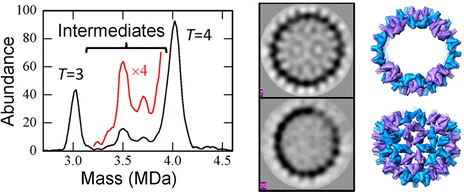
\includegraphics[height=1.35in, width=3.3in]{images/hbvassembly}
\caption{The chart to the left displays an accurate measurement of the
  Hepatitis B virus (HBV) created by the research group's Charge
  Detection Mass Spectrometry research application \cite{247}. This
  detailed mass information is used to create the images shown in the
  middle and to the right, which show 2-D and 3-D models of ions
  within the HBV.}
\label{fig:hbvassembly}
\end{figure}

\subsection{General Problem} \label{problem}
The Martin F. Jarrold research group has the ability to generate a lot
of raw data, all of which needs to be processed by their Fortran
application, as shown in Figure \ref{fig:pipeline}. A typical day
conducting research consists of eight (8) to ten (10) one (1) hour
experiements with each experiement generating raw frequency data at a
rate of four (4) MB/s. Therefore, a single day of experiements has the
ability to generate up to one hundred and forty four (144) GB of
data. The research group must be able to process this data in a
similar amount of time as the time required to generate the raw
data. If their collection of compute resources are not powerful
enough, they will quickly become inundated with piles and piles of raw
data. This day-to-day research workflow typically strains the research
group's local compute resources. Furthermore, the research group
frequently makes algorithmic changes to the CDMS research
application. When a significant change occurs, the research group must
conduct a bulk reprocessing of months or even years worth of raw
data. When a bulk reprocess is required, the limited compute resources
available to the group becomes a significant limitation to the
efficiency of their research. Additionally, when the application is
run on remote sytems, the raw input data must be transfered to the
remote systems and the resulting output must be aggregated and then
plotted in order to visualize and interpret the results. The process
of moving data around by hand is time consuming and the process to
aggregating results is tedious.

\subsection{General Solution} \label{solution}
The research group is composed of domain scientists who do not
necessarily have backgrounds in Computer Science. Therefore, a simple
and reproducible solution must be developed in order to satisfy their
day-to-day research workflow and their bulk reprocessing requirements.

\subsubsection{Cloud Computing}
Leveraging virtual clusters in the cloud to conduct their CDMS
analysis increases their available compute resources while
simultaneously removing the need to manage a collection of compute
resources. The ability to dynamically scale up or down the number of
virutal machines aligns well with the evolving compute needs of the
research group. The software tools Cloudmesh and Ansible Galaxy are at
the backbone of this Cloud Computing solution. These software tools
provide the ability to abstract away the technological details of the
deployment and installation of virtual clusters in the cloud as well
as removes the explicit requirement to run the CDMS application by
hand. These general modifications to their research workflow will
ensure scalability, simplicity and reproducibility, which allows the
domain scientists in the Martin F. Jarrold research group to spend the
majority of their time, effort and money on their research and not on
the technogical hurdles of running the CDMS application.

\begin{figure}
\centering
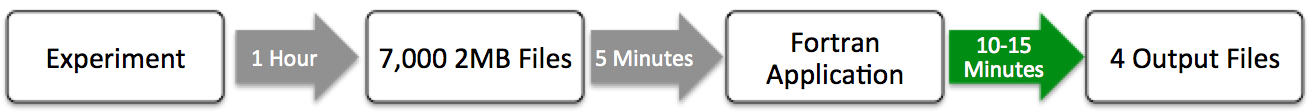
\includegraphics[height=0.45in, width=3.3in]{images/pipeline}
\caption{The Martin F. Jarrold research group's pipeline is shown
  above. This pipeline includes a one (1) hour experiment, which
  creates approximately seven thousand (7,000) two (2) MB raw
  frequency files. Each of these files need to be transfered to the
  remote compute resource(s) and processed with a Fortran application
  to generate four (4) human intrepetable output files.}
\label{fig:pipeline}
\end{figure}

\begin{figure*}[h]
\centering
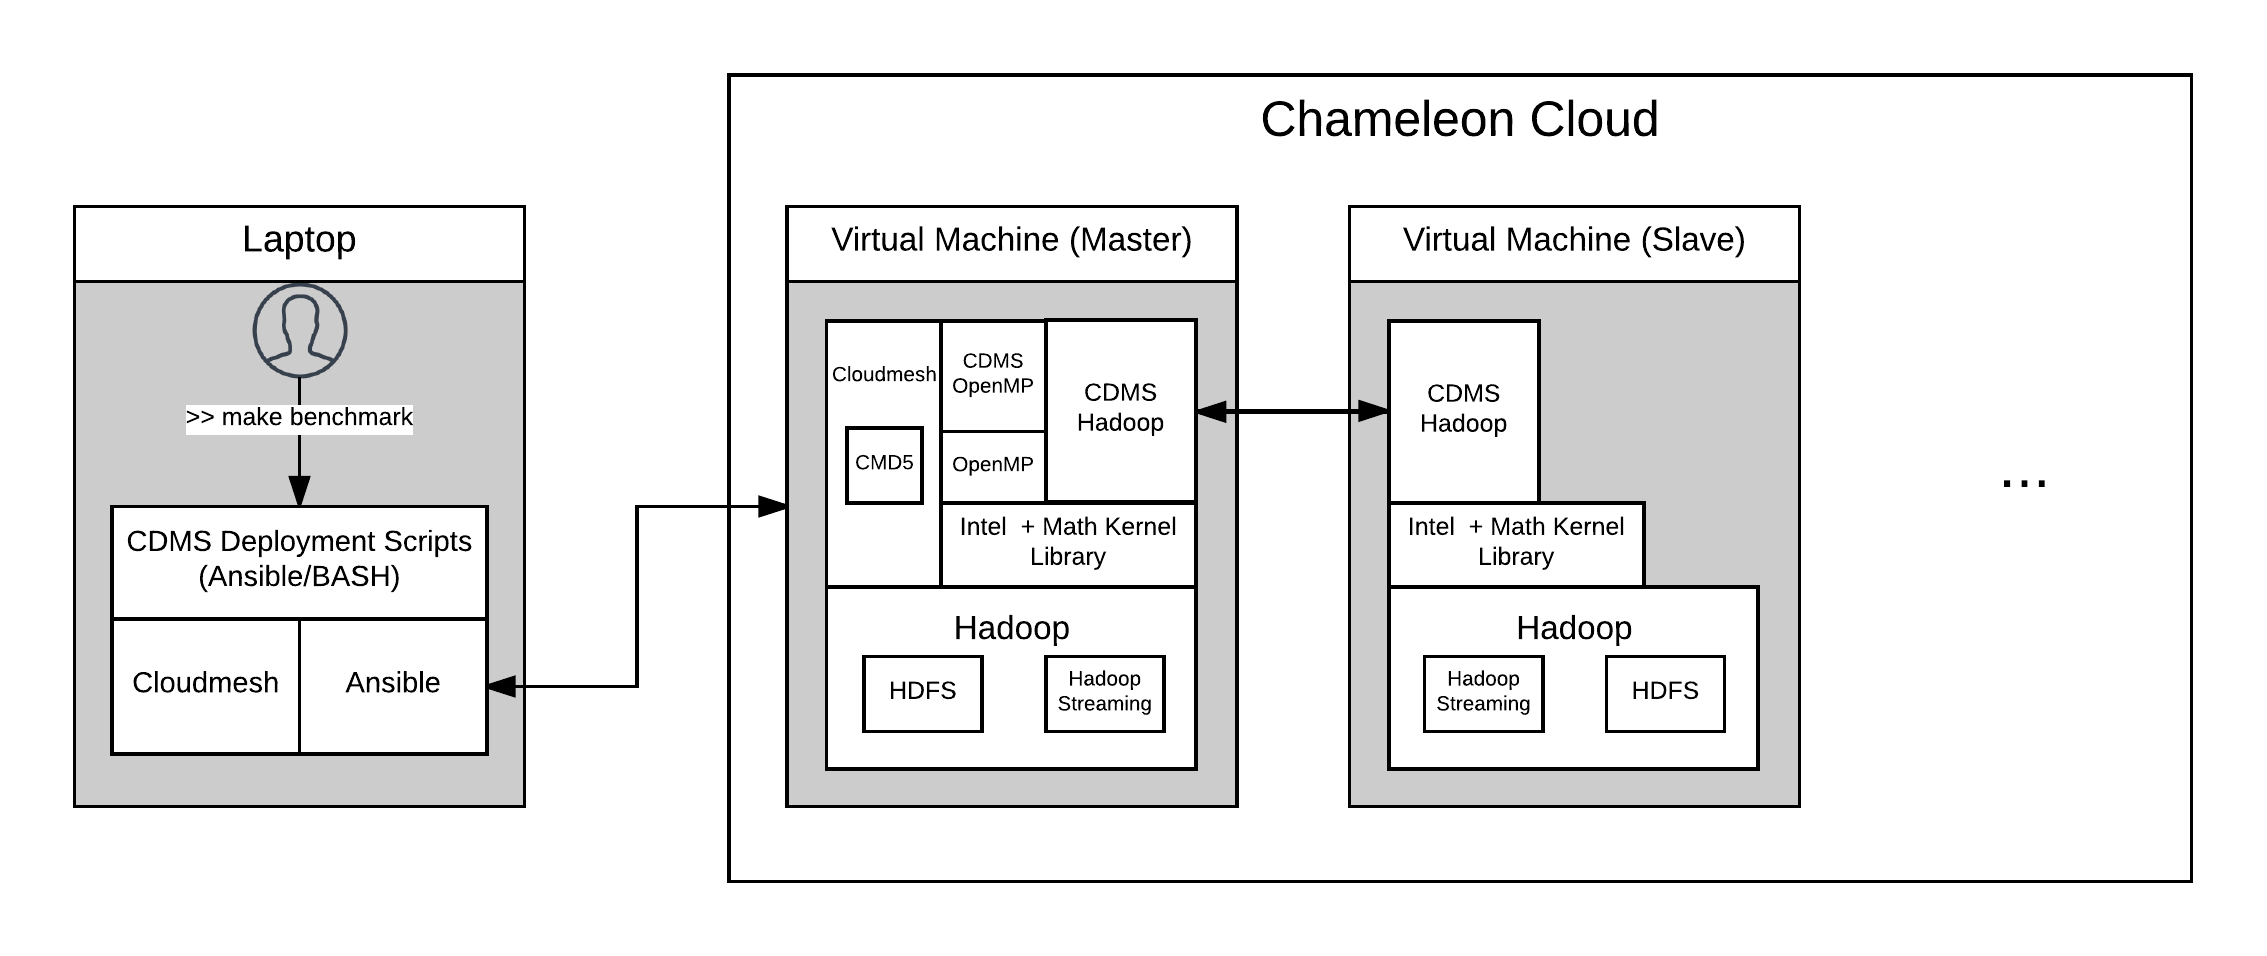
\includegraphics[height=3.0in, width=\textwidth]{images/architecture}
\caption{The figure above provides a visual representation of the
  underlying architecture required for the Charge Detection Mass
  Spectrometry Cloud Computing workflow. The necessary software
  (i.e. Cloudmesh, Ansible, Hadoop, Intel, and etc.) and compute
  resources (i.e. Laptop and Virtual Machines) are explicitly shown
  above.}
\end{figure*}

\section{Architecture} \label{architecture}
The underlying architecture of this cloud computing research workflow
is explicity designed to facilitate automation. Cloudmesh and Ansible
Galaxy are the main software tools that enable the creation of the
virtual cluster, the deployment of software/data and the execution of
the CDMS research application.

\subsection{Software} \label{software}
\subsubsection{Cloudmesh Client Toolkit} 
The Cloudmesh Client Toolkit provides an application programming
interface (API), which enables users to simply manage a set of cloud
resources (i.e. virtual machines, virtual clusters and etc.)
\cite{cloudmesh}. The Cloudmesh Client Toolkit abstracts away the
technological details of managing Cloud Computing resources.

\subsubsection{Ansible Galaxy} 
Ansible is an information technology automation service designed for
software deployment and execution \cite{ansible}.  Ansible Galaxy is
an Ansible community, which``provides pre-packaged units of work known
to Ansible as roles'' \cite{ansible-galaxy}. Ansible Galaxy's
pre-packaged units of work are essentially shared solutions to common
automation tasks. This is a representation of open source style of the
Ansible Galaxy community. Ansible Galaxy promotes fast development
since the wheel does not need to be reinvented for the automation of
common tasks.

\subsubsection{CDMS Application} 
The Martin F. Jarrold Group has written a Fast Fourier based
application written in Fortran in order to conduct their CDMS
research. This application is composed of approximately fifteen
thousand (15,000) lines of Fortran code. Depending on the input, about
60\% to 70\% of the total compute time is spent within the external
Intel Math Kernal Library (MKL) conducting the required Fast Fourier
Transformations (FFT).

\subsubsection{Intel} 
The CDMS source code is compiled with the Intel compiler. The CDMS
application relies on the Math Kernel Library (MKL) to leverage
efficient Fast Fourier Computations. The application also leverages
the Intel OpenMP parallel framework in order to divide the work
amongst available CPU's. Therefore, the Intel software is a
fundamental piece of the architecture, which provides the compiler,
MKL, and OpenMP functionality.

\subsubsection{Hadoop} 
Apache Hadoop ``is a framework that allows for the distributed
processing of large data sets across clusters of computers using
simple programming models'' \cite{hadoop}. Therefore, Hadoop must be
installed at the foundation of each virtual machine in the cloud in
order to leverage multiple virtual machines during the CDMS processing
phase of the workflow.

\subsection{Data} \label{data}
The CDMS application requires a set of raw two (2) MB files as
input. In order to develop and test the efficiency of the deployment,
a small dataset was used to generate all of the performance
results. This small test dataset, composed of two hundred (200) files
has a total size of four hundred (400) MB and is a representative
sample. A typical dataset for the research group is approximately
fourteen (14) GB in size. In a single day, up to ten (10) datasets are
created and need to be processed.

\section{Licensing} \label{licensing}
\subsection{CDMS Deployment Scripts} \label{source-license}
The source code (i.e. Bash, Ansible, Python) presented here is
licensed under the Apache License, Version 2.0 \cite{www-apache-lic}.

\subsection{CDMS Application} \label{cdms-license}
The Martin F. Jarrold Group research group owns all of the rights to
the Fortran Source code and data. All distribution of the application
and data must be consented by the research group.

\subsection{Intel} \label{intel-license}
The Intel software requires a license in order to complete the
installation. A student license is obtainable for free with an
\emph{EDU} email address; however, the leveraginng the Indiana
University Intel license server would provide a more complete and
reproducible solution. In order to use the Indiana University Intel
license server, the Virtual Machines must reside in the Indiana
University IP address space. This can be achieved by connecting each
virtual machine to Indiana University's Virtual Private Network
(i.e. VPN). In order to connect to the VPN, one must connect via DUO
Authentication (i.e. use a phone or token to validate). Given the
complexity and reliability concerns with connecting to Indiana
University's VPN, the free Intel student license was selected in order
to promote reproducibility.

\subsubsection{Student License Limitations} \label{student-license}
The CDMS Deployment Scripts that were developed for this project
leverage a free Intel student license to compile and link the CDMS
application. While anyone can use this student license, this license
is registered to the author of this paper. This student license is
\emph{System Locked} and therefore can be installed on at most five
(5) virutal machines. Once this threshold has been passed, the Intel
software (i.e compiler, MKL and OpenMP) can no longer be
installed. This limitatation inhibits the reproducibility and
scalability of the research workflow. If a license registration error
occurs during the Intel build phase of the deployment of the software,
please contact the author of this paper. The author has the ability to
uninstall the license from the registered hosts using Intel's
Registration Center website \cite{intel-reg}.

\section{Parallelization} \label{parallel}
The Charge Detection Mass Spectrometry input data is split into many
two (2) MB files. Conveniently, the data within each file is entirely
independent to the data in the other input files. Therefore, the input
data files can be processed simultaneously or in parallel. Parallel
processing may not seem important when working on our sample dataset
composed of two hundred (200) files; however, when a large collection
of data requires reprocessing, parallel processing becomes critical to
the Martin F. Jarrold research group.
\subsection{OpenMP}
OpenMP is a shared memory parallelization framework that is specified
with simple compiler directives \cite{openmp}. The shared memory
parallelization structure limits the scalability of the application to
a single node or virtual machine. This is in contrast to distributed
memory parallelization, such as Message Passing Interface (MPI) or
Hadoop, which enables multi-node parallelization \cite{mpi,
  hadoop}. The original developers of the CDMS application decided to
leverage OpenMP parallelization in order to exploit the natural data
independency and improve overall performance of the application.
\subsection{Hadoop}
In order to improve the overall performance significantly, a
distributed processing framework such as Hadoop must be integrated
into the CDMS application. This would allow for parallelization across
multiple virtual machines in the CDMS application.  The source code is
composed of fifteen thousand (15,000) lines of Fortran code that
interfaces with the Intel Math Kernel Library. In order to leverage
the Hadoop API, the source code would need to be rewritten in a
compatible programming language such as Java or Python.
\subsubsection{Hadoop Streaming}
Hadoop Streaming provides an alternative to rewriting the application
in a compatible programming language. Hadoop Streaming allows one to
``create and run Map/Reduce jobs with any executable or script as the
mapper and/or the reducer''
\cite{https://hadoop.apache.org/docs/r1.2.1/streaming.html}.  The only
modifcation that was needed to use Hadoop Streaming in the CDMS
application was alter the way in which the data was inputted to the
application and outputted from the application. In Hadoop Streaming,
``the mapper and the reducer are executables that read the input from
stdin (line by line) and emit the output to stdout''
\cite{hadoop-streaming}. The overall structure of the application and
its data allowed for a straightforward transformation from OpenMP
parallelization Hadoop Streaming parallelization, as shown in Figure
\ref{fig:hadoop}. The application natively reads the input and writes
the output to text files. Modifying the application to read from stdin
and write to stdout allowed for the integration of Hadoop Streaming.
\begin{figure}[h]
\centering
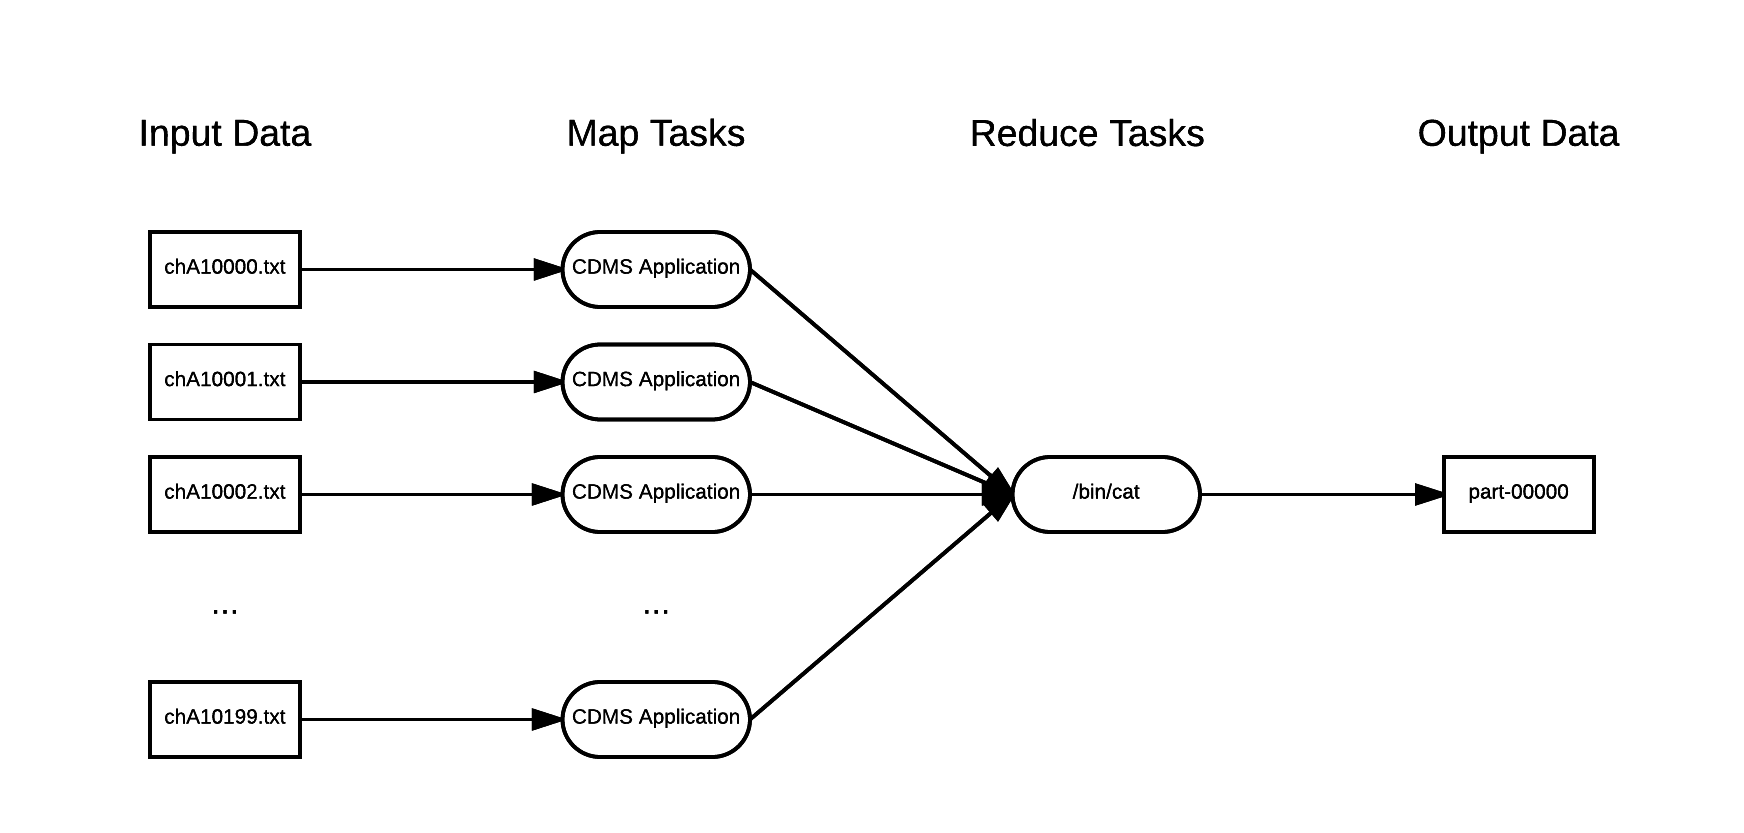
\includegraphics[height=1.65in, width=\columnwidth]{images/mapreduce}
\caption{The diagram shown above indicates the MapReduce style
  analysis of the CDMS Hadoop Streaming version of the
  application. Each input file is processed indpendently and the
  results are aggregated with a single \emph{cat} reduce task.}
\label{fig:hadoop}
\end{figure}

\section{Getting Started}
The CDMS Deployment Scripts were specifically designed to promote
reproduciblility. The following subsections describe how to use the
CDMS Deployment Scripts to install and run the CDMS application in the
cloud with as little as one simple command.
\subsection{Requirements} \label{req}
In order to execute the CDMS Deployment Scripts, one must have the
Cloudmesh Client and Ansible installed on their local
system. Additionally, a valid $\sim$/.cloudmesh/cloudmesh.yaml
configuration file must be stored locally.
\subsection{Fetch Code} \label{git}
The CDMS Deployment Scripts are hosted using Github
\cite{i524-github}. This repository contains the required Ansible and
Bash scripts used to launch the research workflow.
\noindent See the following Bash commands:
\begin{lstlisting}[language=bash]
  >> git clone [REPOSITORY]
  >> cd sp17-i524/project/S17-IO-3011/code
\end{lstlisting}
\subsection{Benchmark} \label{benchmark-info}
A single command will deploy the Hadoop virtual cluster, install the
required software, run the three versions (i.e. Serial, OpenMP and
Hadoop Streaming) of the CDMS application, aggregate the results,
create plots of the output and delete the Hadoop virtual
cluster. Timing information for each of these stages is printed to the
screen once the benchmark has completed. The performance of this
benchmark is plotted and explained in Section \ref{performance}.
\noindent See the following Bash command:
\begin{lstlisting}[language=bash]
  >> make benchmark
\end{lstlisting}
By default the benchmark will be run on one, two and three virtual
machines. You can modify the maximum number of virtual machines
(i.e. 5) to be used in the benchmark by passing in an optional
argument to the \emph{benchmark} Makefile option. The example shown
below will run the benchmark with one, two, three, four and five
virtual machines.
\noindent See the following Bash command:
\begin{lstlisting}[language=bash]
  >> make benchmark num_nodes=5
\end{lstlisting}
\subsection{Additional Commands} \label{other}
In case one would like to break up the aforementioned benchmark into
individual pieces, there are seperate Bash commands available.
\noindent See the following Bash commands:
\begin{lstlisting}[language=bash]
  >> make deploy [num_nodes=x]
  >> make install
  >> make run
  >> make view
  >> make delete
  >> make clean
\end{lstlisting}
\subsubsection{Deploy}
The \emph{deploy} Makefile option leverages Cloudmesh to deploy a
Hadoop virutal cluster in the Chameleon Cloud. By default three (3)
virtual machines will be created with the \emph{deploy} option. The
specific number of virtual machines deployed can be configured by
passing in num\_nodes=x, where x is the number of virutal machines
requested to be deployed in the virtual cluster.
\subsubsection{Install}
The \emph{install} Makefile option installs necessary software
(i.e. Intel Compiler, Intel MKL, Python, Pip, Cloudmesh, Git, Charge
Detection Mass Spectrometry application, and etc.) on the master and
slave virtual machines of the active virtual cluster.
\subsubsection{Run}
The \emph{run} Makefile option runs the serial, OpenMP, and Hadoop
Streaming versions of the CDMS application on the active virtual
cluster using the small test dataset containing two hundred (200)
input files.
\subsubsection{View}
The \emph{view} Makefile option aggregates the output data from the
virtual machines in the active cluster, plots the results using
Python's matplotlib and transfers a subset of the plots to the local
system in order to visually validate the accuracy of the application.
\subsubsection{Delete}
The \emph{delete} Makefile option deletes all virtual machines
associated with ones username in the cloud.
\subsubsection{Clean}
The \emph{clean} Makefile option removes all local output files, if
they exist.

\section{Compute Resources} \label{resources}
The CDMS OpenMP parallel application was tested on multiple compute
resources, as explained in Section \ref{performance}. Each resource
has unique qualities that impact the performance, scalability and
degree of parallelism. 
\subsection{Windows HPC Server}
The Martin F. Jarrold's local Windows HPC Server has eight (8)
CPUs. Therefore, the Charge Detection Mass Spectrometry OpenMP
application can process up to eight (8) input files in parallel.
\subsection{Karst}
Indiana University's Supercomputer, named Karst, has sixteen (16) CPUs
per node. Therefore, the Charge Detection Mass Spectrometry
application can processs up to sixteen (16) input files in parallel.
\subsection{Big Red II}
Indiana University's Supercomputer, named Big Red II, has thirty two
(32) CPUs per node. Therefore, the Charge Detection Mass Spectrometry
OpenMP application can processs up to thirty two (32) input files in
parallel.
\subsection{Chameleon Cloud}
Cloudmesh allows one to specify different flavors of virutal machines
to be deployed in the Chameleon Cloud. These flavors come in various
sizes (i.e. Memory, vCPUs, and etc.). As shown in Table
\ref{tab:hadoop}, these flavors can be used strategically to specify
the number of virtual CPUs used in the virtual machine. In this case,
the Chameleon Cloud m1.xlarge flavor provides eight (8) vCPUs. This
allows the Charge Detection Mass Spectrometry OpenMP application to
process up to eight (8) input files in parallel.
\begin{table}[htbp]
\centering
\begin{tabular}{cc}
\multicolumn{2}{c}{\bf Chameleon Cloud Virtual Machine Flavors}\\
\hline
\# Flavor & \# of vCPUs \\
\hline
m1.medium & 2 \\
m1.large & 4 \\
m1.xlarge & 8 \\
\hline
\end{tabular}
\caption{The table above indicates the number of virtual CPUs
  allocated to the various Virtual Machine flavors in the Chameleon
  Cloud. The number of vCPUs indicate the maximum degree of
  parallelism for the CDMS application.}
\label{tab:hadoop}
\end{table}

\section{Performance Results} \label{performance}
As discussed in Section \ref{code}, the application is parallelized
using OpenMP. Therefore, this application utilizes the avaialable
computational power available. Figure \ref{fig:scalability2} compares
the performance of the application on difference compute resources
(i.e. local servers, Supercomputers and clouds).

The time required to deploy and run the application in the cloud is
shown in the figure \ref{fig:benchmark}. This benchmark includes the
time required for the installation of the software subsystems as well
as the time required to run the application.
\subsection{OpenMP Scalability} \label{omp-scalability}
The Charge Detection Mass Spectrometry OpenMP version of the
application performs well when the compute resources increase, as
shown in Figure \ref{fig:scalability2}. The application performs most
efficiently on Karst when using sixteen (16) CPUs (i.e. 16 OpenMP
threads). However, when the application is run using one (1), two (2),
four (4) or eight (8) CPUs, the best performance exists on the
Chameleon Cloud, as shown in Figure
\ref{fig:scalability2}. Specifically, the application performs 18\%
faster on a single Chameleon Cloud virutal machine when compared to
running the application on eight (8) CPUs of Karst. 
\begin{figure}[h]
\centering
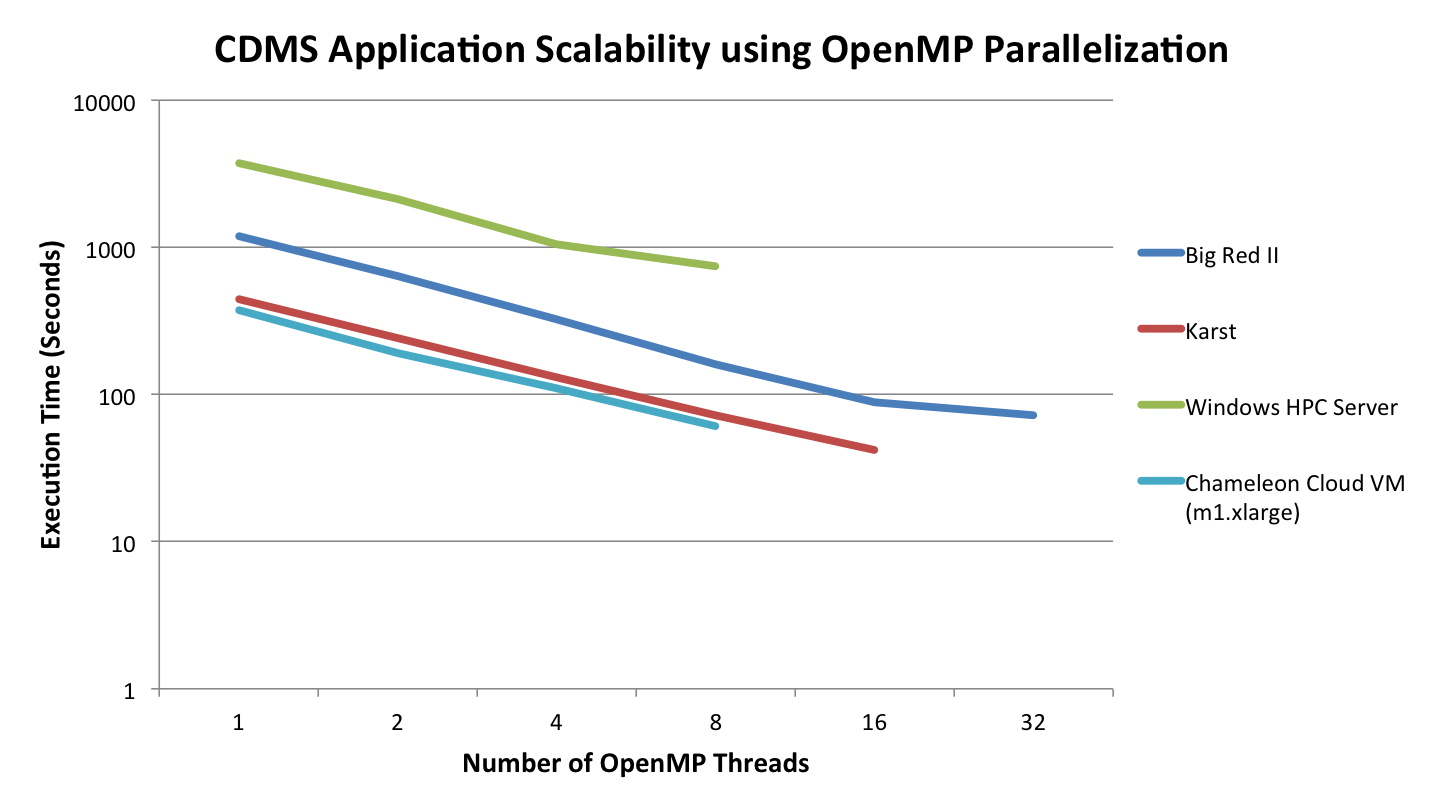
\includegraphics[height=2.1in, width=3.3in]{images/scalability2}
\caption{The figure above shows the scalability (i.e. reduction in
  time-to-solution) as the number of OpenMP threads increase on local
  servers, Supercomputers and Clouds.}
\label{fig:scalability2}
\end{figure}

\subsection{Hadoop Scalability} \label{hadoop-scalability}
The Hadoop Streaming application does not exhibit the desired
scalability. Since the application is essentially a map only Hadoop
application, the performance (i.e. total runtime) of the application
should decrease linearly with an increase in the number of nodes
deployed. However, the performance results in Table \ref{tab:hadoop}
indicate that the runtime remains relatively consistent when one (1),
two (2) or three (3) virtual machines are used to process the two
hundred (200) raw input data files. The performance analysis of the
Hadoop Streaming application will be conducted as part of the Future
Work, as explain in Section \ref{future}.

\begin{figure}[h]
\centering
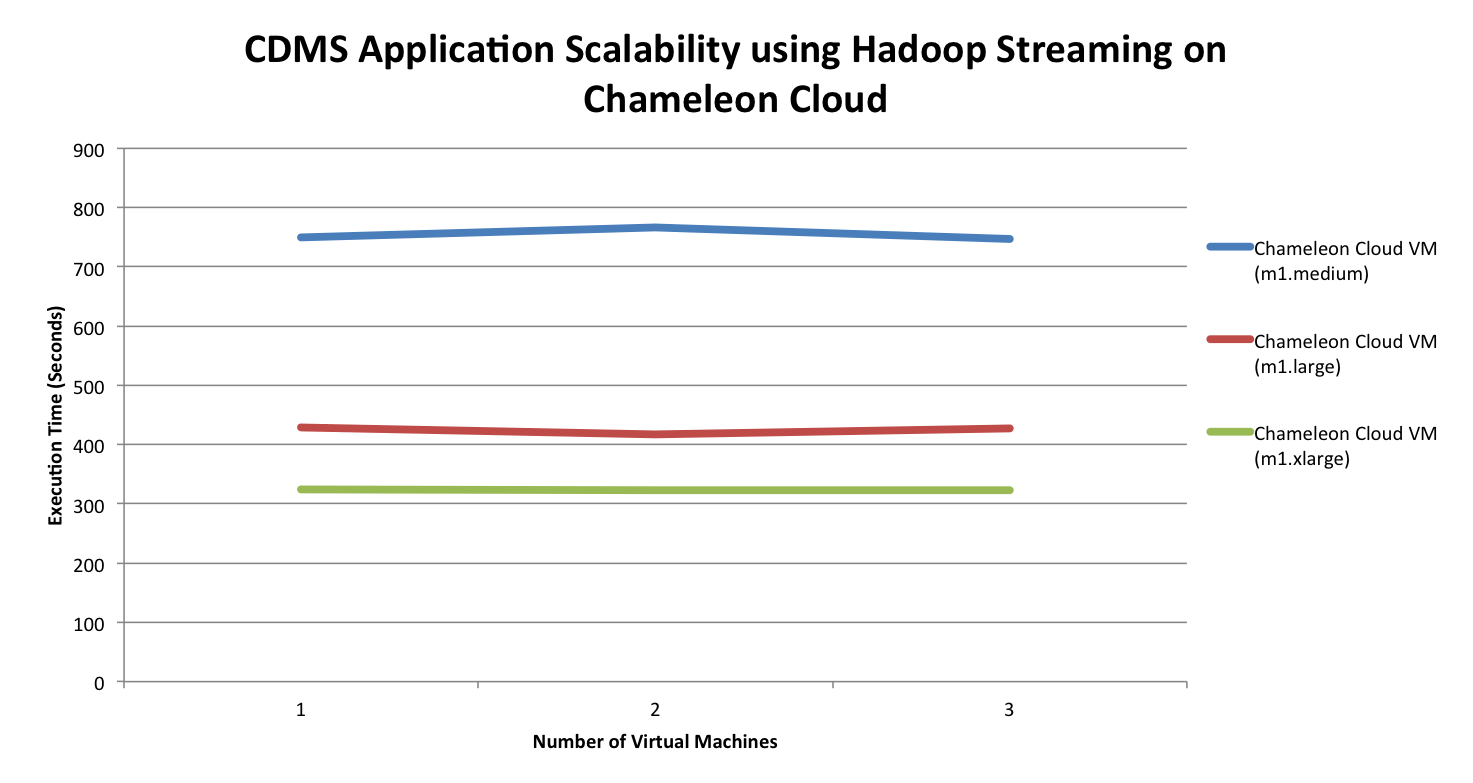
\includegraphics[height=2.1in, width=3.3in]{images/hadoop_benchmark}
\caption{The table above shows the scalability (i.e. reduction in
  time-to-solution) of the Charge Detection Mass Spectrometry Hadoop
  Streaming application as the number of Virtual Machines increase in
  the Chameleon Cloud Cluster.}
\label{fig:benchmark}
\end{figure}

\subsection{Full Benchmark Scalability} 
Interestingly, the full benchmark including deploying the virutal
machines, installing the required software, running the serial, OpenMP
and Hadoop Streaming version of the CDMS application, and
aggregating/plotting the results was tested using one (1), two (2) and
three (3) virutal machines in the Chameleon Cloud. Interestingly, the
benchmark required more and more time as the number of virtual
machines increased. This performance information indicates that the
deployment overhead outweighs the potential benefits of leveraging
multiple virtual machines. The lack of scalability shown in the Hadoop
Streaming version of the application also inhibits the runtime.
\begin{figure}[h]
\centering
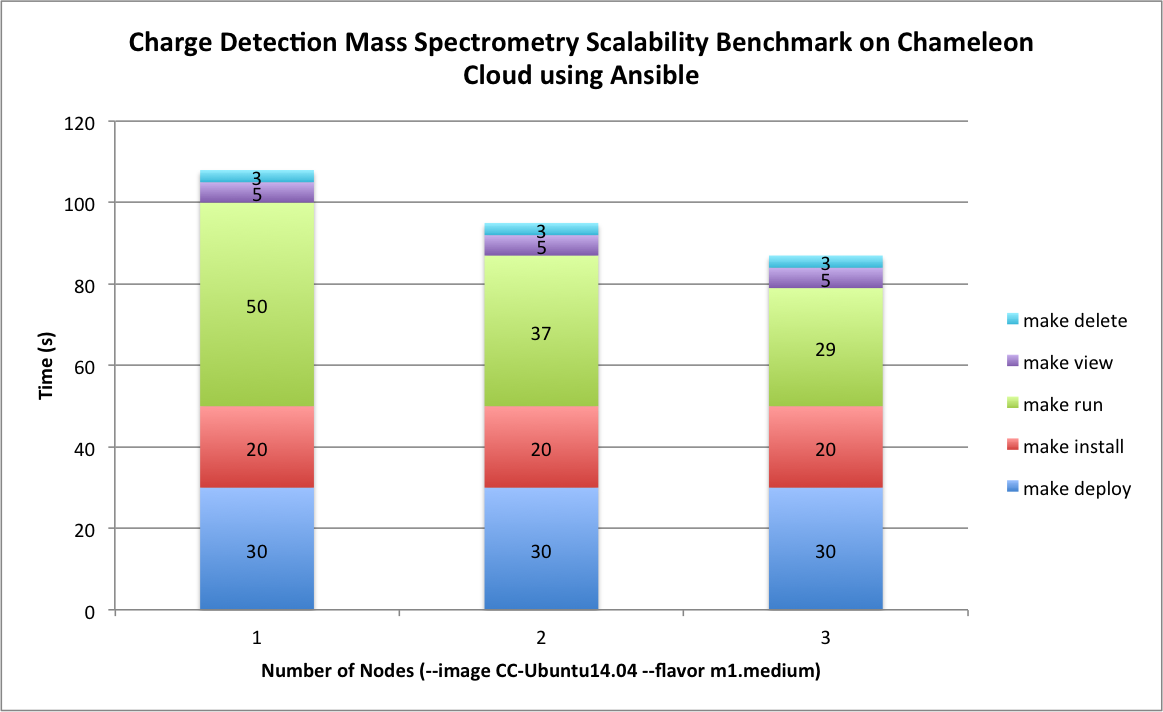
\includegraphics[height=2.1in, width=3.3in]{images/benchmark}
\caption{The figure above indicates the time-to-solution for a full
  benchmark of the deployment of one (1), two (2) and three (3)
  virutal machines in the Chameleon Cloud. This benchmark includes
  depoying the virtual machines, installing all software, running the
  serial, OpenMP and Hadoop Streaming versions of the application and
  aggregating/plotting the results.}
\label{fig:benchmark}
\end{figure}


\section{Future Work} \label{future}
Future work includes analyzing the performance of the CDMS Hadoop
Streaming application to understand the poor scalability when running
on multiple nodes.  Future work on this project includes using larger
images and more virtual machines in order to increase the performance
of the Hadoop Streaming application. Future work includes figuring out
how to leverage Indiana University's Intel license server. This will
increase reproducibility by allowing the Intel Compiler and Intel MKL
to be installed on an unlimited number of virutal machines. Future
work includes dispersing the raw input data across multiple virutal
machines and running an instance of the CDMS OpenMP application on
each virutal machine and then aggregating the results. Future work
includes integrating Message Passing Interface (MPI) as the parallelel
backbone of the application rather than OpenMP. This will increase the
scalability of the application to more than a single virtual machine.

\section{Conclusion} \label{conclusion}
The use of the Cloudmesh Client and Ansible Galaxy software to
automate the execution of the Charge Detection Mass Spectrometry
research application in the cloud imporved the simplicity, efficiency
and reproducibility. The automation allows the Martin F. Jarrold
research group to focus on the details of their specific research
rather than on the details of managing the software subsystems,
executing the application and managing the input/output data. This
automated Cloud Computing solution benefits the Martin F. Jarrold
research group with respect to both simplicity and performance of the
application. Streamelining the research workflow will inevitably
result in an increase in productivity for the research group. An
increase in research productivity may also result in an increase in
grant funding and/or an increase in publications for the Indiana
University research group.

The performance of the CDMS OpenMP version of the application
performed favorably on a single Chameleon Cloud virtual machine when
compared with a single node of the Indiana University High Performance
Computing clusters (e.g. Karst and Big Red II). This unexpected result
has sparked furture work in optimizing the OpenMP version of the
application for the Chameleon Cloud. However, the overhead included
with deploying the virtual cluster and installing the necessary
software causes the overall time-to-solution to increase dramatically.

The Hadoop Streaming version of the CDMS application did not exhibit
optimal performance on the Chameleon Cloud virtual cluster. If the
execution time reduced when more virtual machines were used, then this
version of the application would become a viable solution for the
research group's need to bulk reprocess raw input data. The Hadoop
streaming CDMS version of the application is a step in the right
direction; however, additional work must to be done to ensure
scalability across multiple virtual machines.

\section*{Acknowledgements}
The authors would like to thank the School of Informatics and
Computing for providing the Big Data Software and Projects (INFO-I524)
course \cite{www-i524}. This project would not have been possible
without the technical support \& edification from Gregor von Laszewski
and his distinguished colleagues.

 
\section*{Author Biographies}
\begingroup
\setlength\intextsep{0pt}
\begin{minipage}[t][3.2cm][t]{1.0\columnwidth} 
  \begin{wrapfigure}{L}{0.25\columnwidth}
    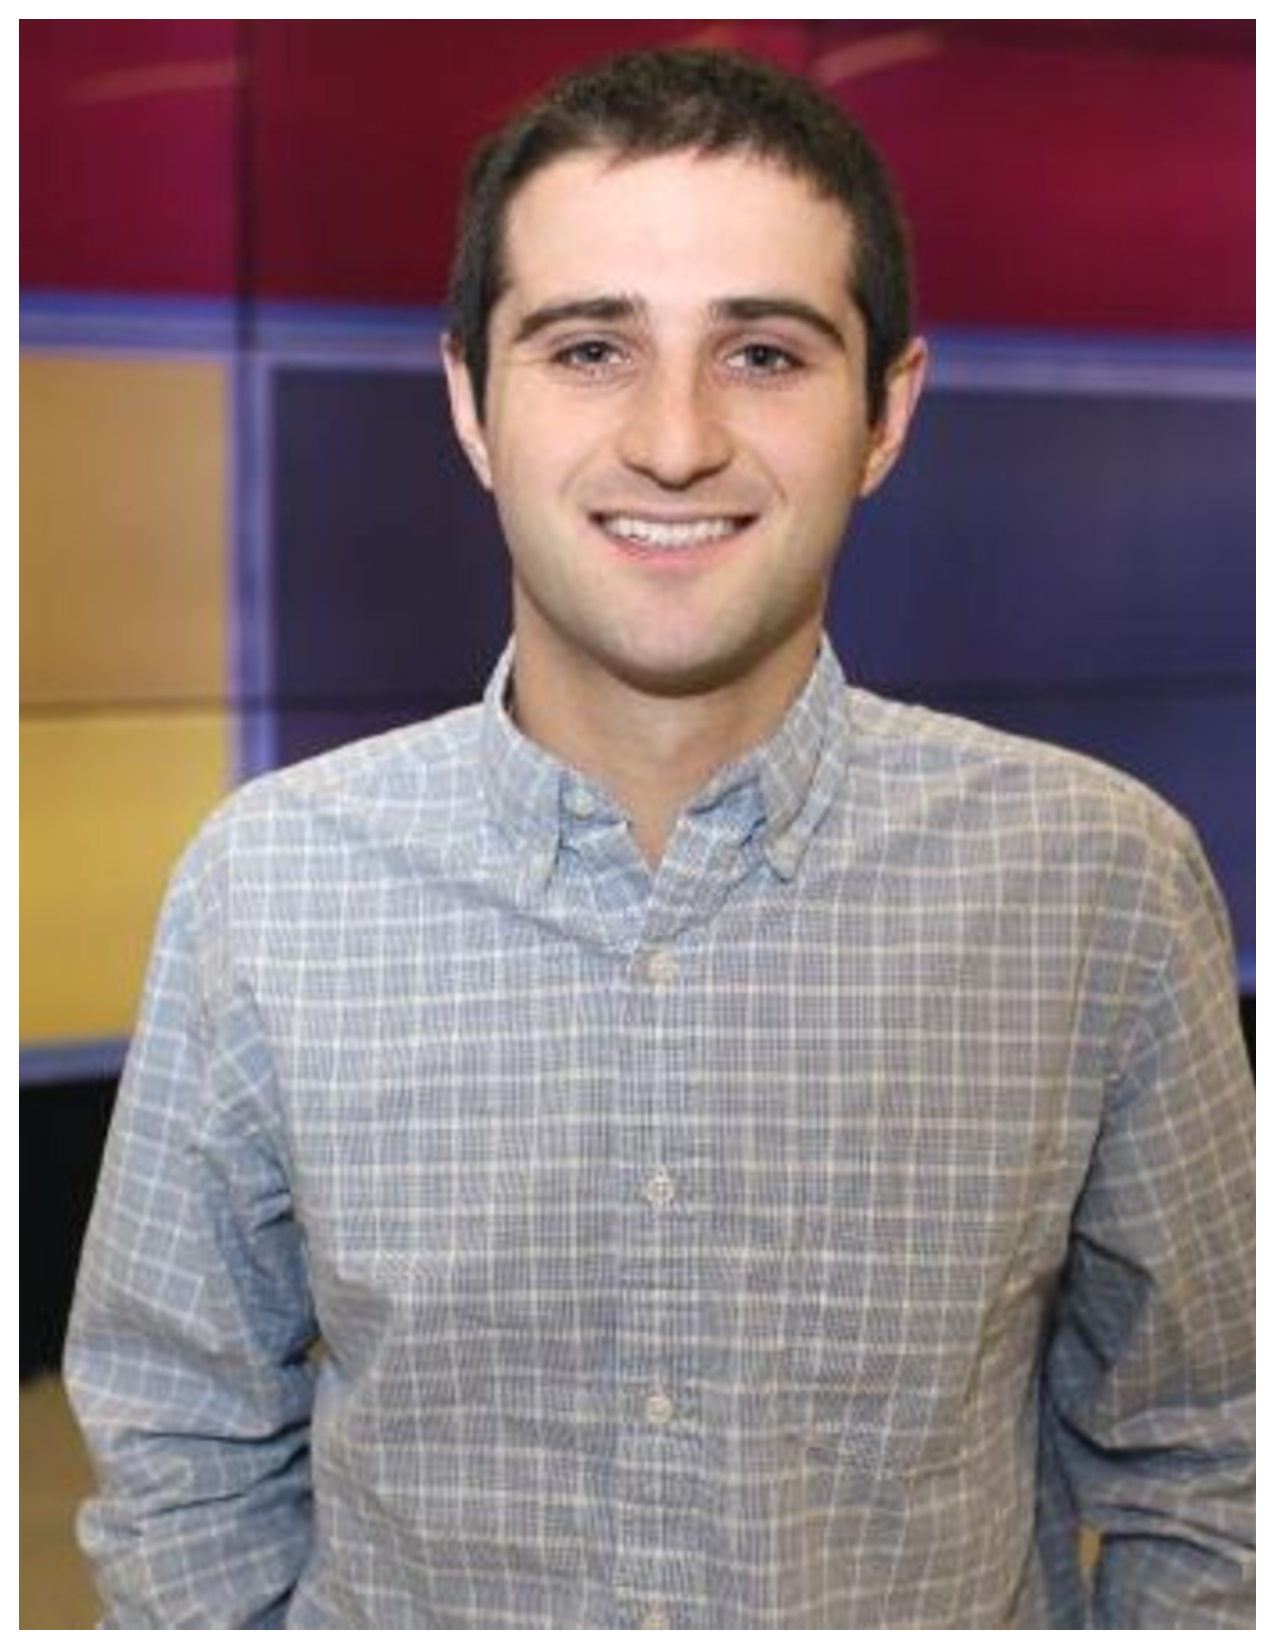
\includegraphics[width=0.25\columnwidth]{images/scott_mcclary}
  \end{wrapfigure}
  \noindent
  {\bfseries Scott McClary} received his BSc (Computer Science) and
  Minor (Mathematics) in May 2016 from Indiana University and will
  receive his MSc (Computer Science) in May 2017 from Indiana
  University. His research interests are within scientific application
  performance analysis on large-scale HPC systems. He will begin
  working as a Software Engineer with General Electric Digital in San
  Ramon, CA in July 2017.
\end{minipage}
\endgroup

\section*{} %used to create more spacing..
\section*{Work Breakdown}
The work on this project was distributed as follows between the
authors:
\begin{description}
\item[Scott McClary.] He completed all of the work for this project
  including researching, deploying, testing and benchmarking the
  Charge Detection Mass Spectrometry research application as well as
  composing this paper.
\end{description}

% Bibliography
\bibliography{references}
\end{document}

